\chapter{Implementation}\label{ch:implementation}

This chapter introduces some interesting implementation details and techniques, focusing mainly on the frontend but also mentioning the backend, including the spaced repetition algorithm.


\section{Frontend implementation}

This section presents the completed frontend application, illustrated with pictures, and then describes the solutions used during the implementation, highlighting the exciting features.

\subsection{The frontend application and screenshots}

This subsection presents the key interfaces of the SpacedAce platform. The screenshots illustrate the main user interactions and core functionalities.

The first figure~\ref{fig:screenshot-quizzes} illustrates the application's main page, the \textbf{My quizzes} page, where the user can see the quizzes and manage them.

\begin{figure}[H]
	\centering
	\frame{
		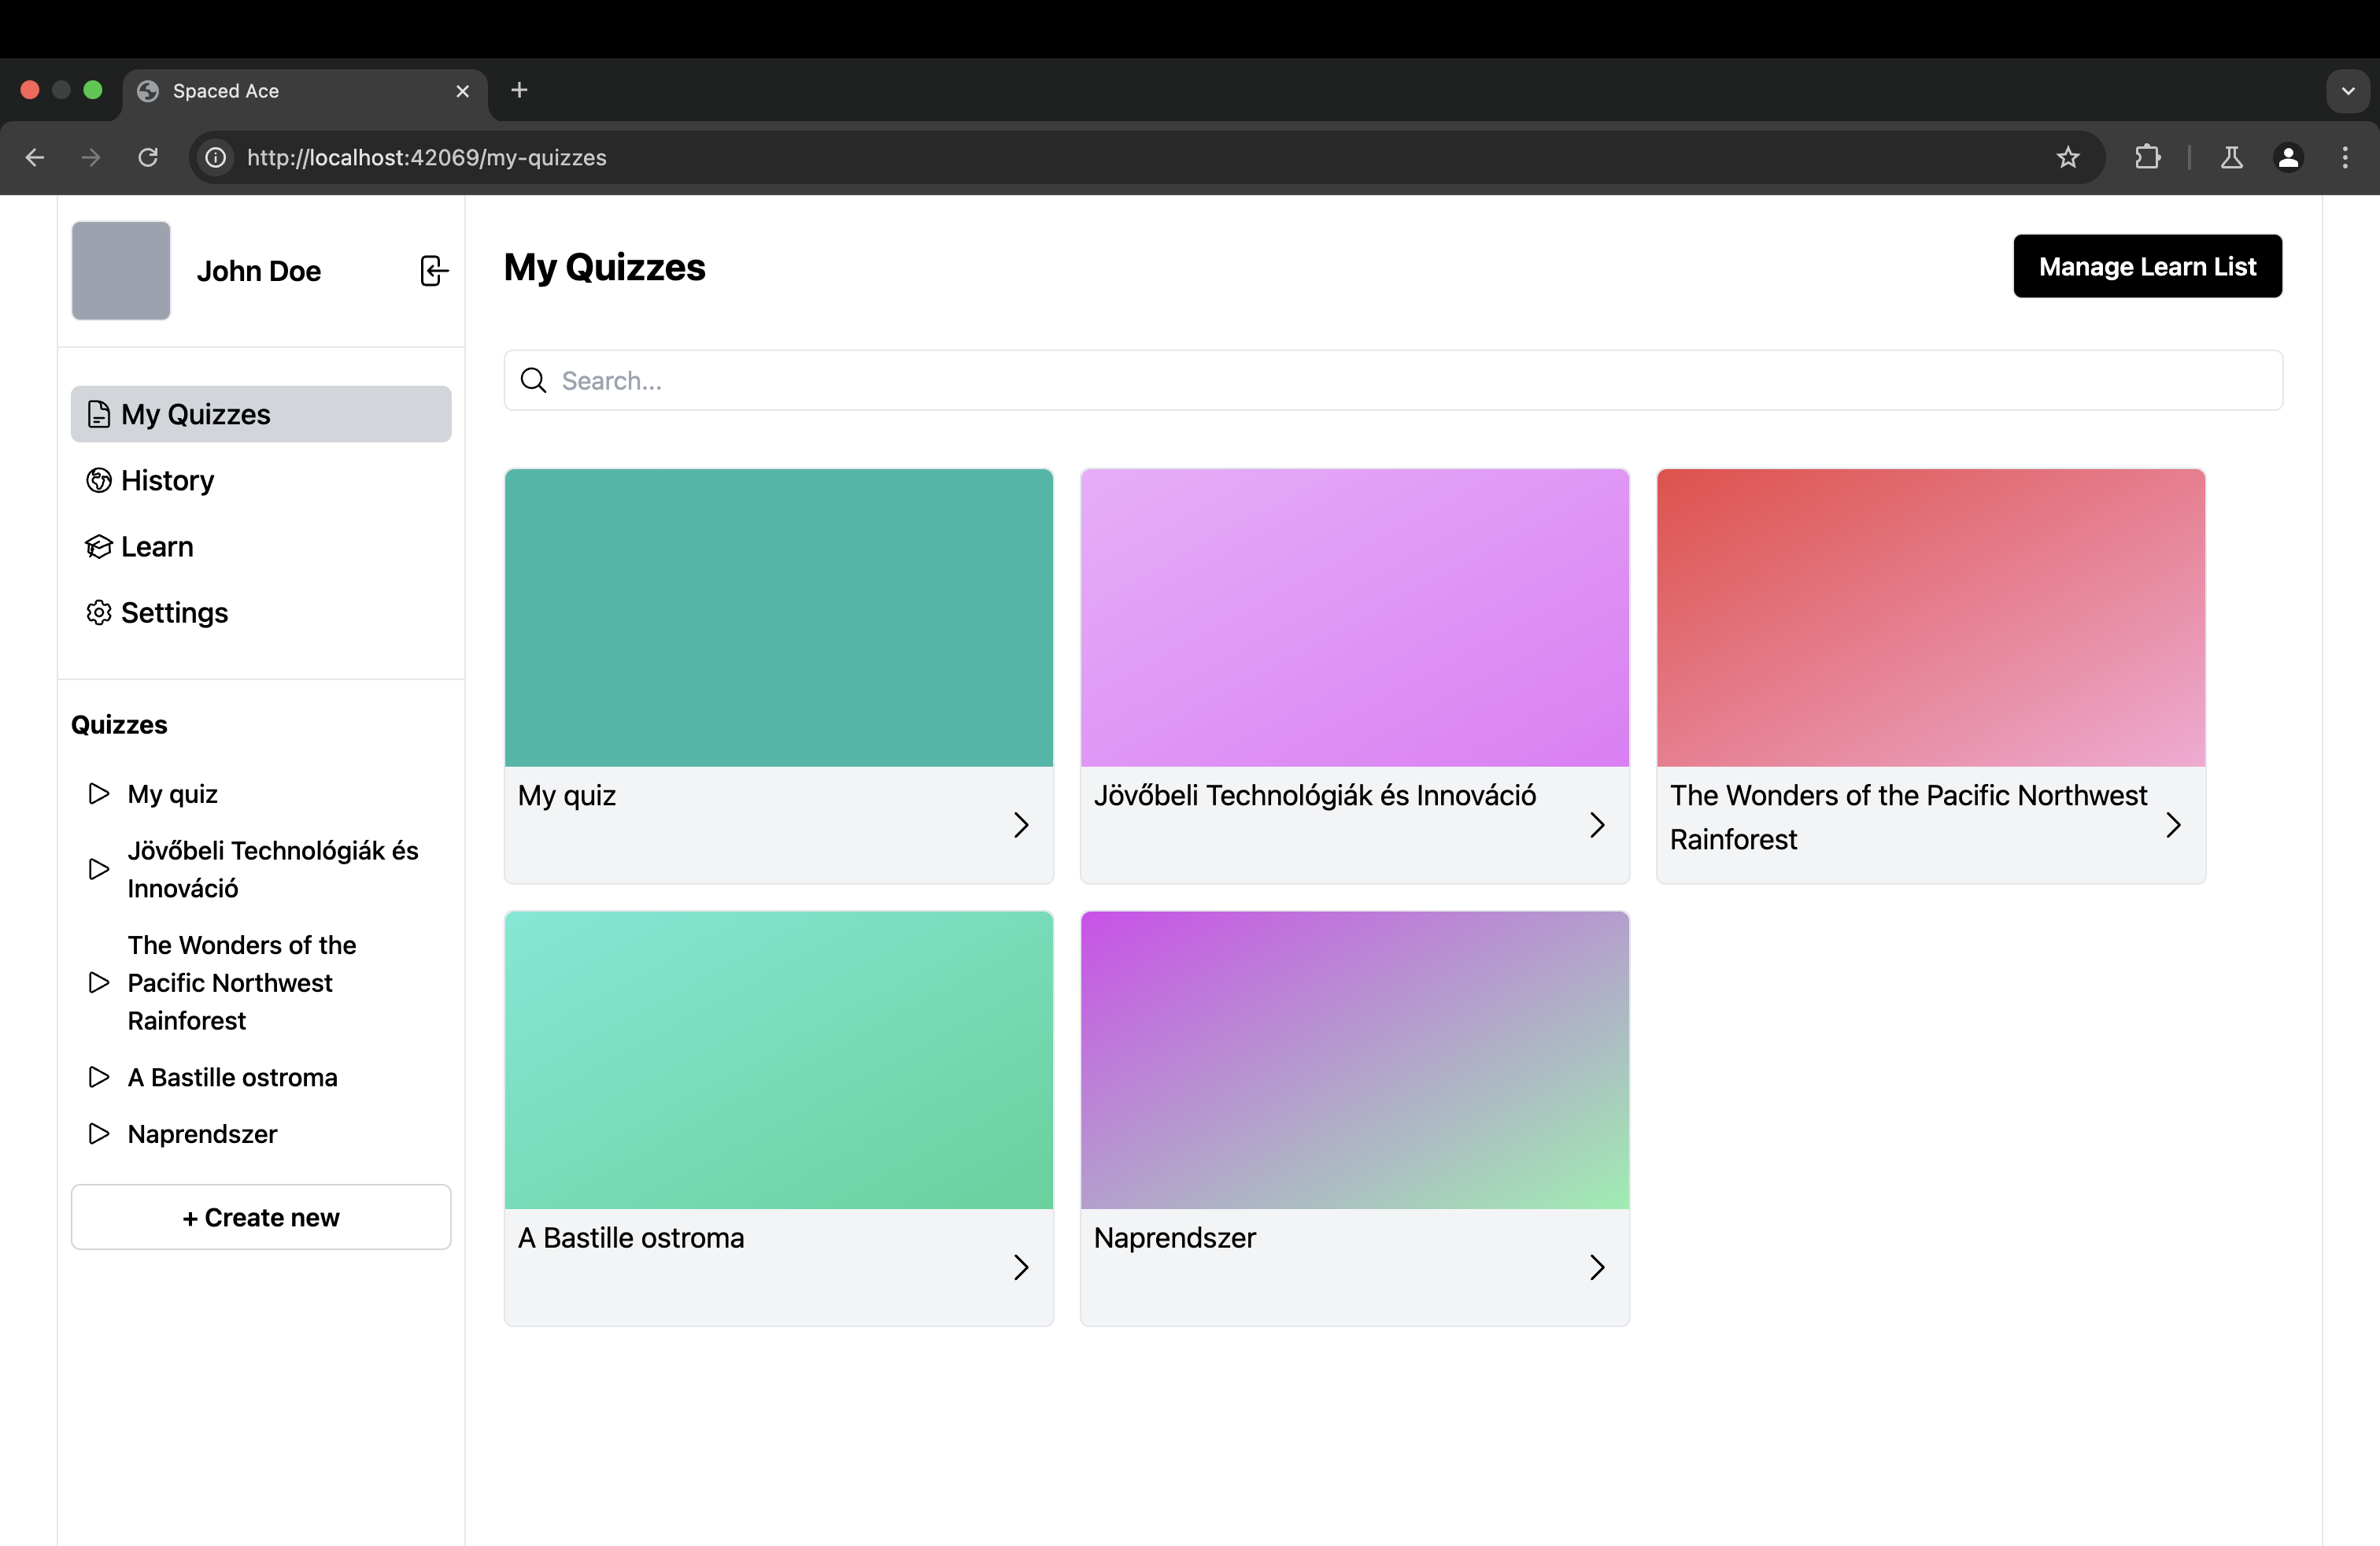
\includegraphics[width=0.9\textwidth, keepaspectratio]{figures/screenshot-quizzes.png}
	}
	\caption{My quizzes page}
	\label{fig:screenshot-quizzes}
\end{figure}

The second figure~\ref {fig:screenshot-question-generation} uses the platform's question generation function.

\begin{figure}[H]
	\centering
	\frame{
		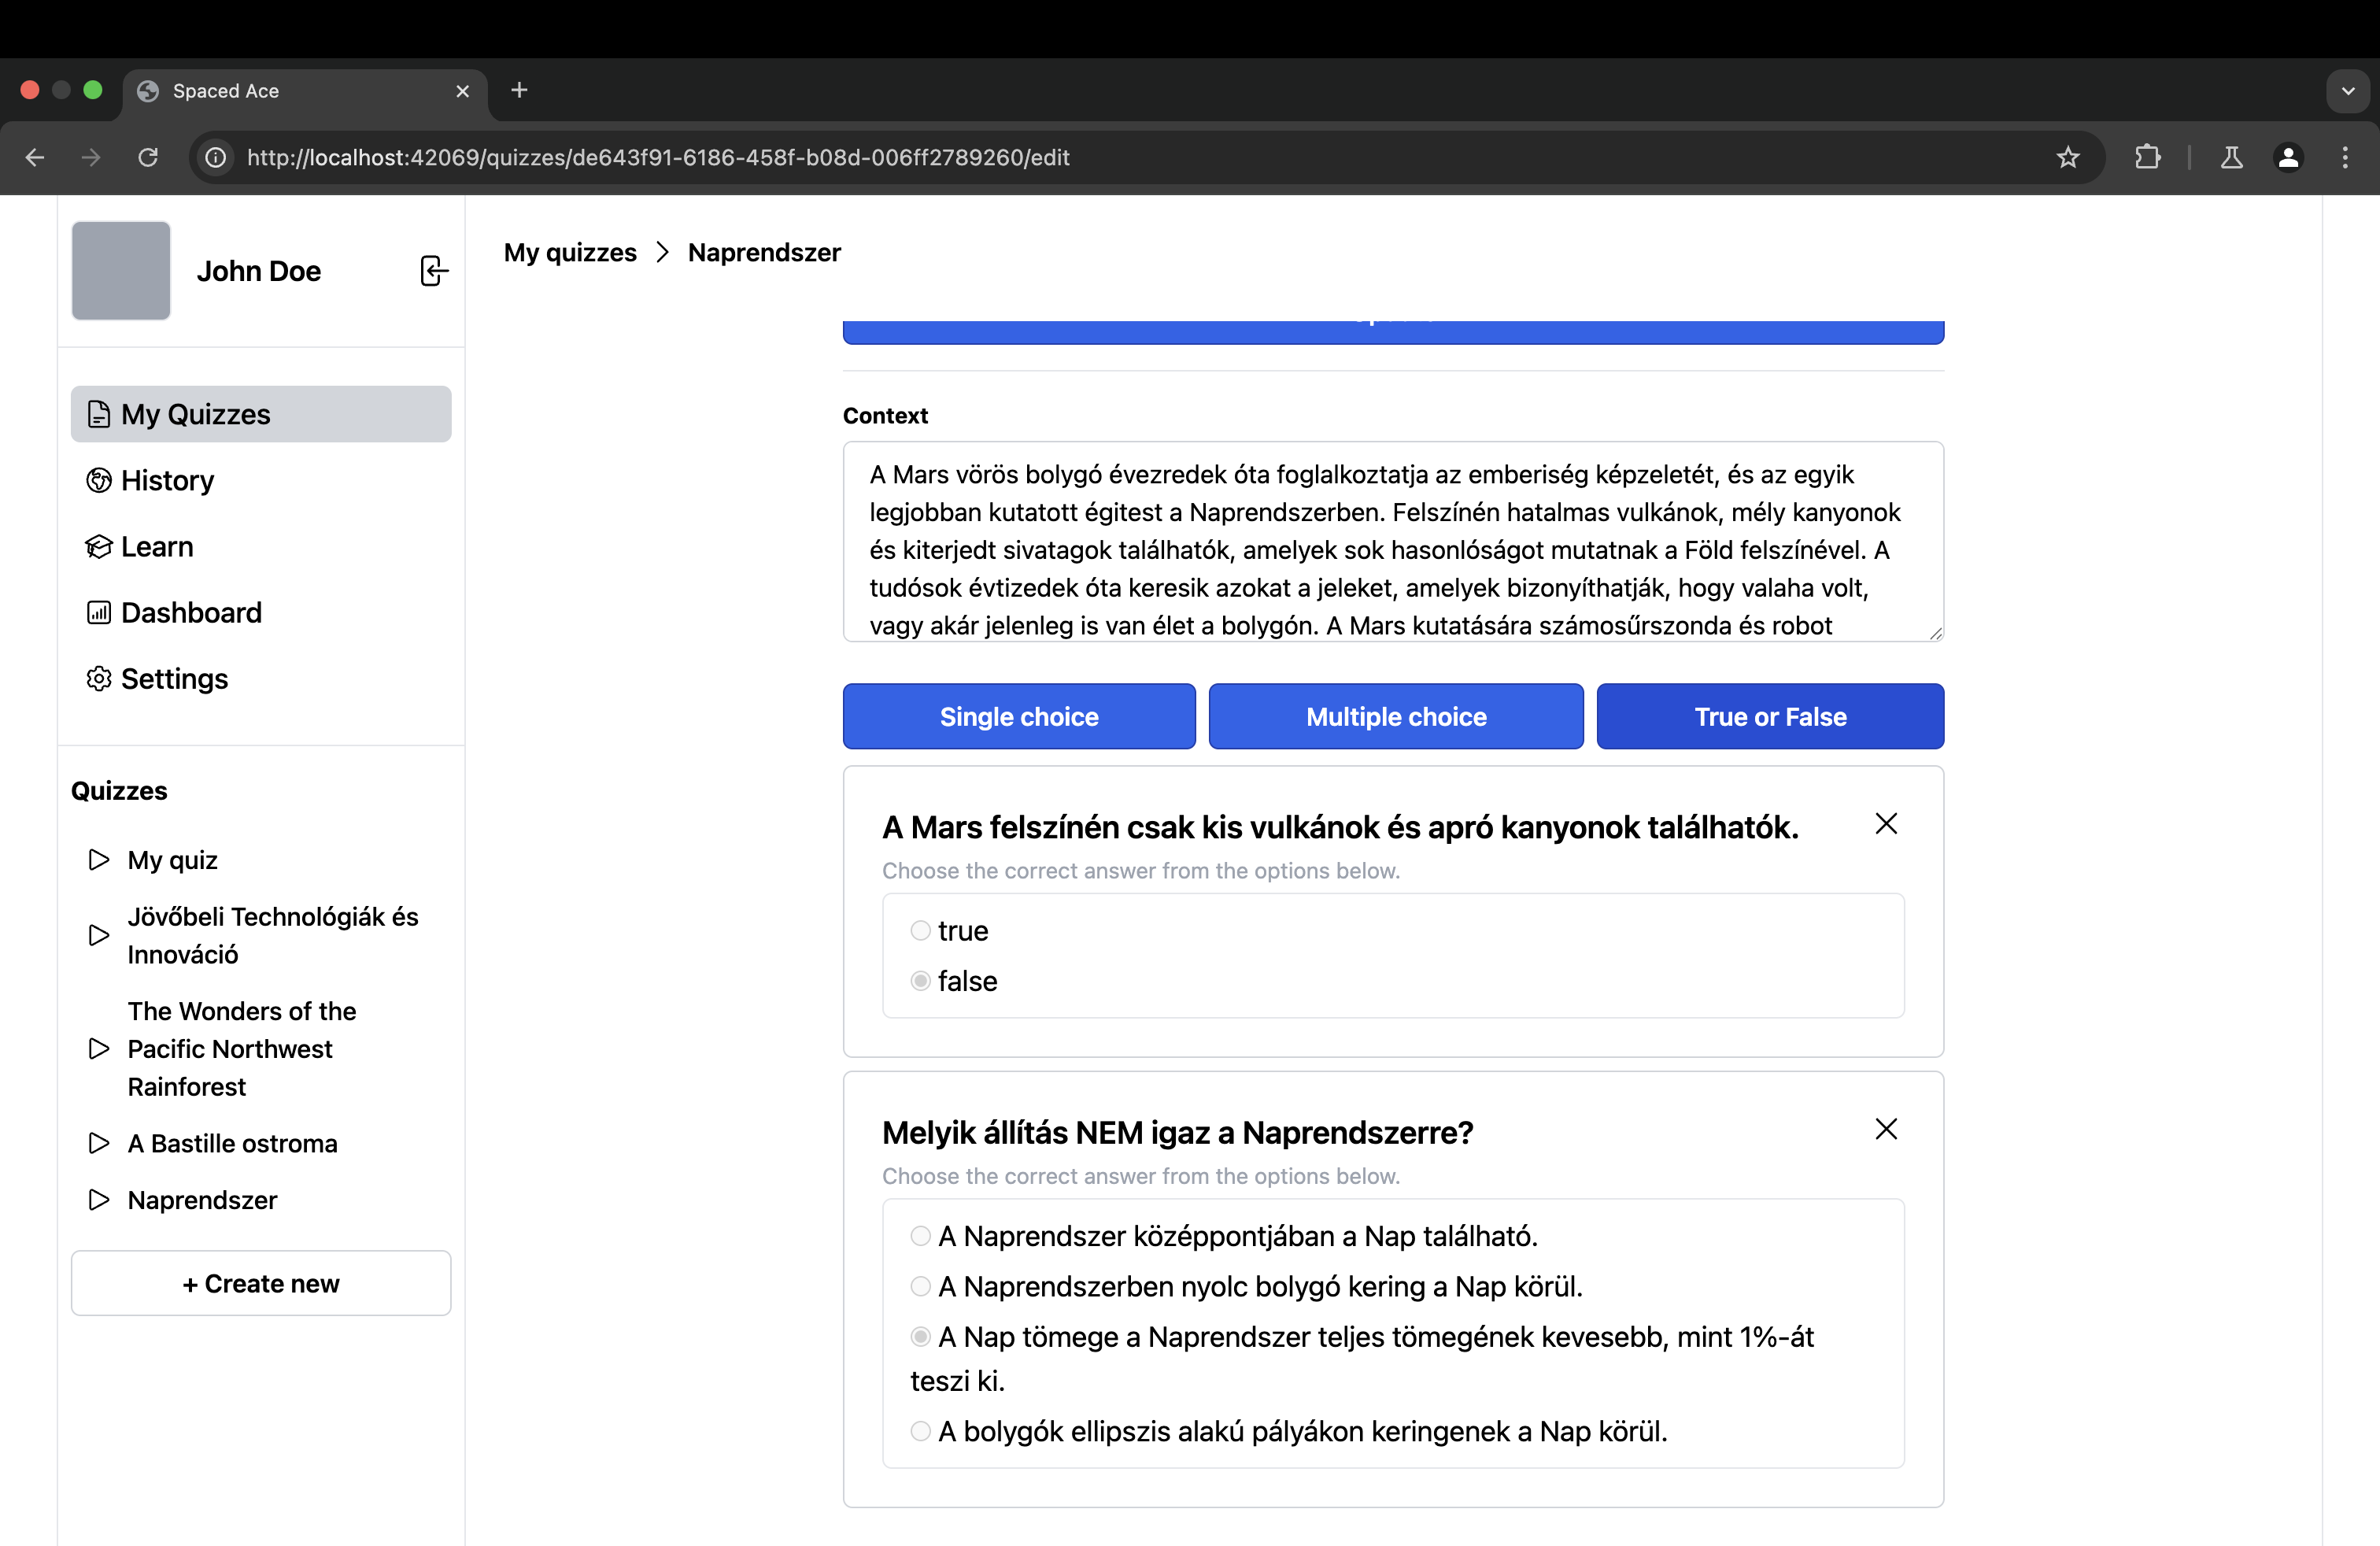
\includegraphics[width=0.9\textwidth, keepaspectratio]{figures/screenshot-question-generation.png}
	}
	\caption{Question generation}
	\label{fig:screenshot-question-generation}
\end{figure}

The last figure~\ref{fig:screenshot-learn-page} in the subsection illustrates the \textbf{Learn} page, where the user can see the scheduled questions done by the spaced repetition algorithm.

\begin{figure}[H]
	\centering
	\frame{
		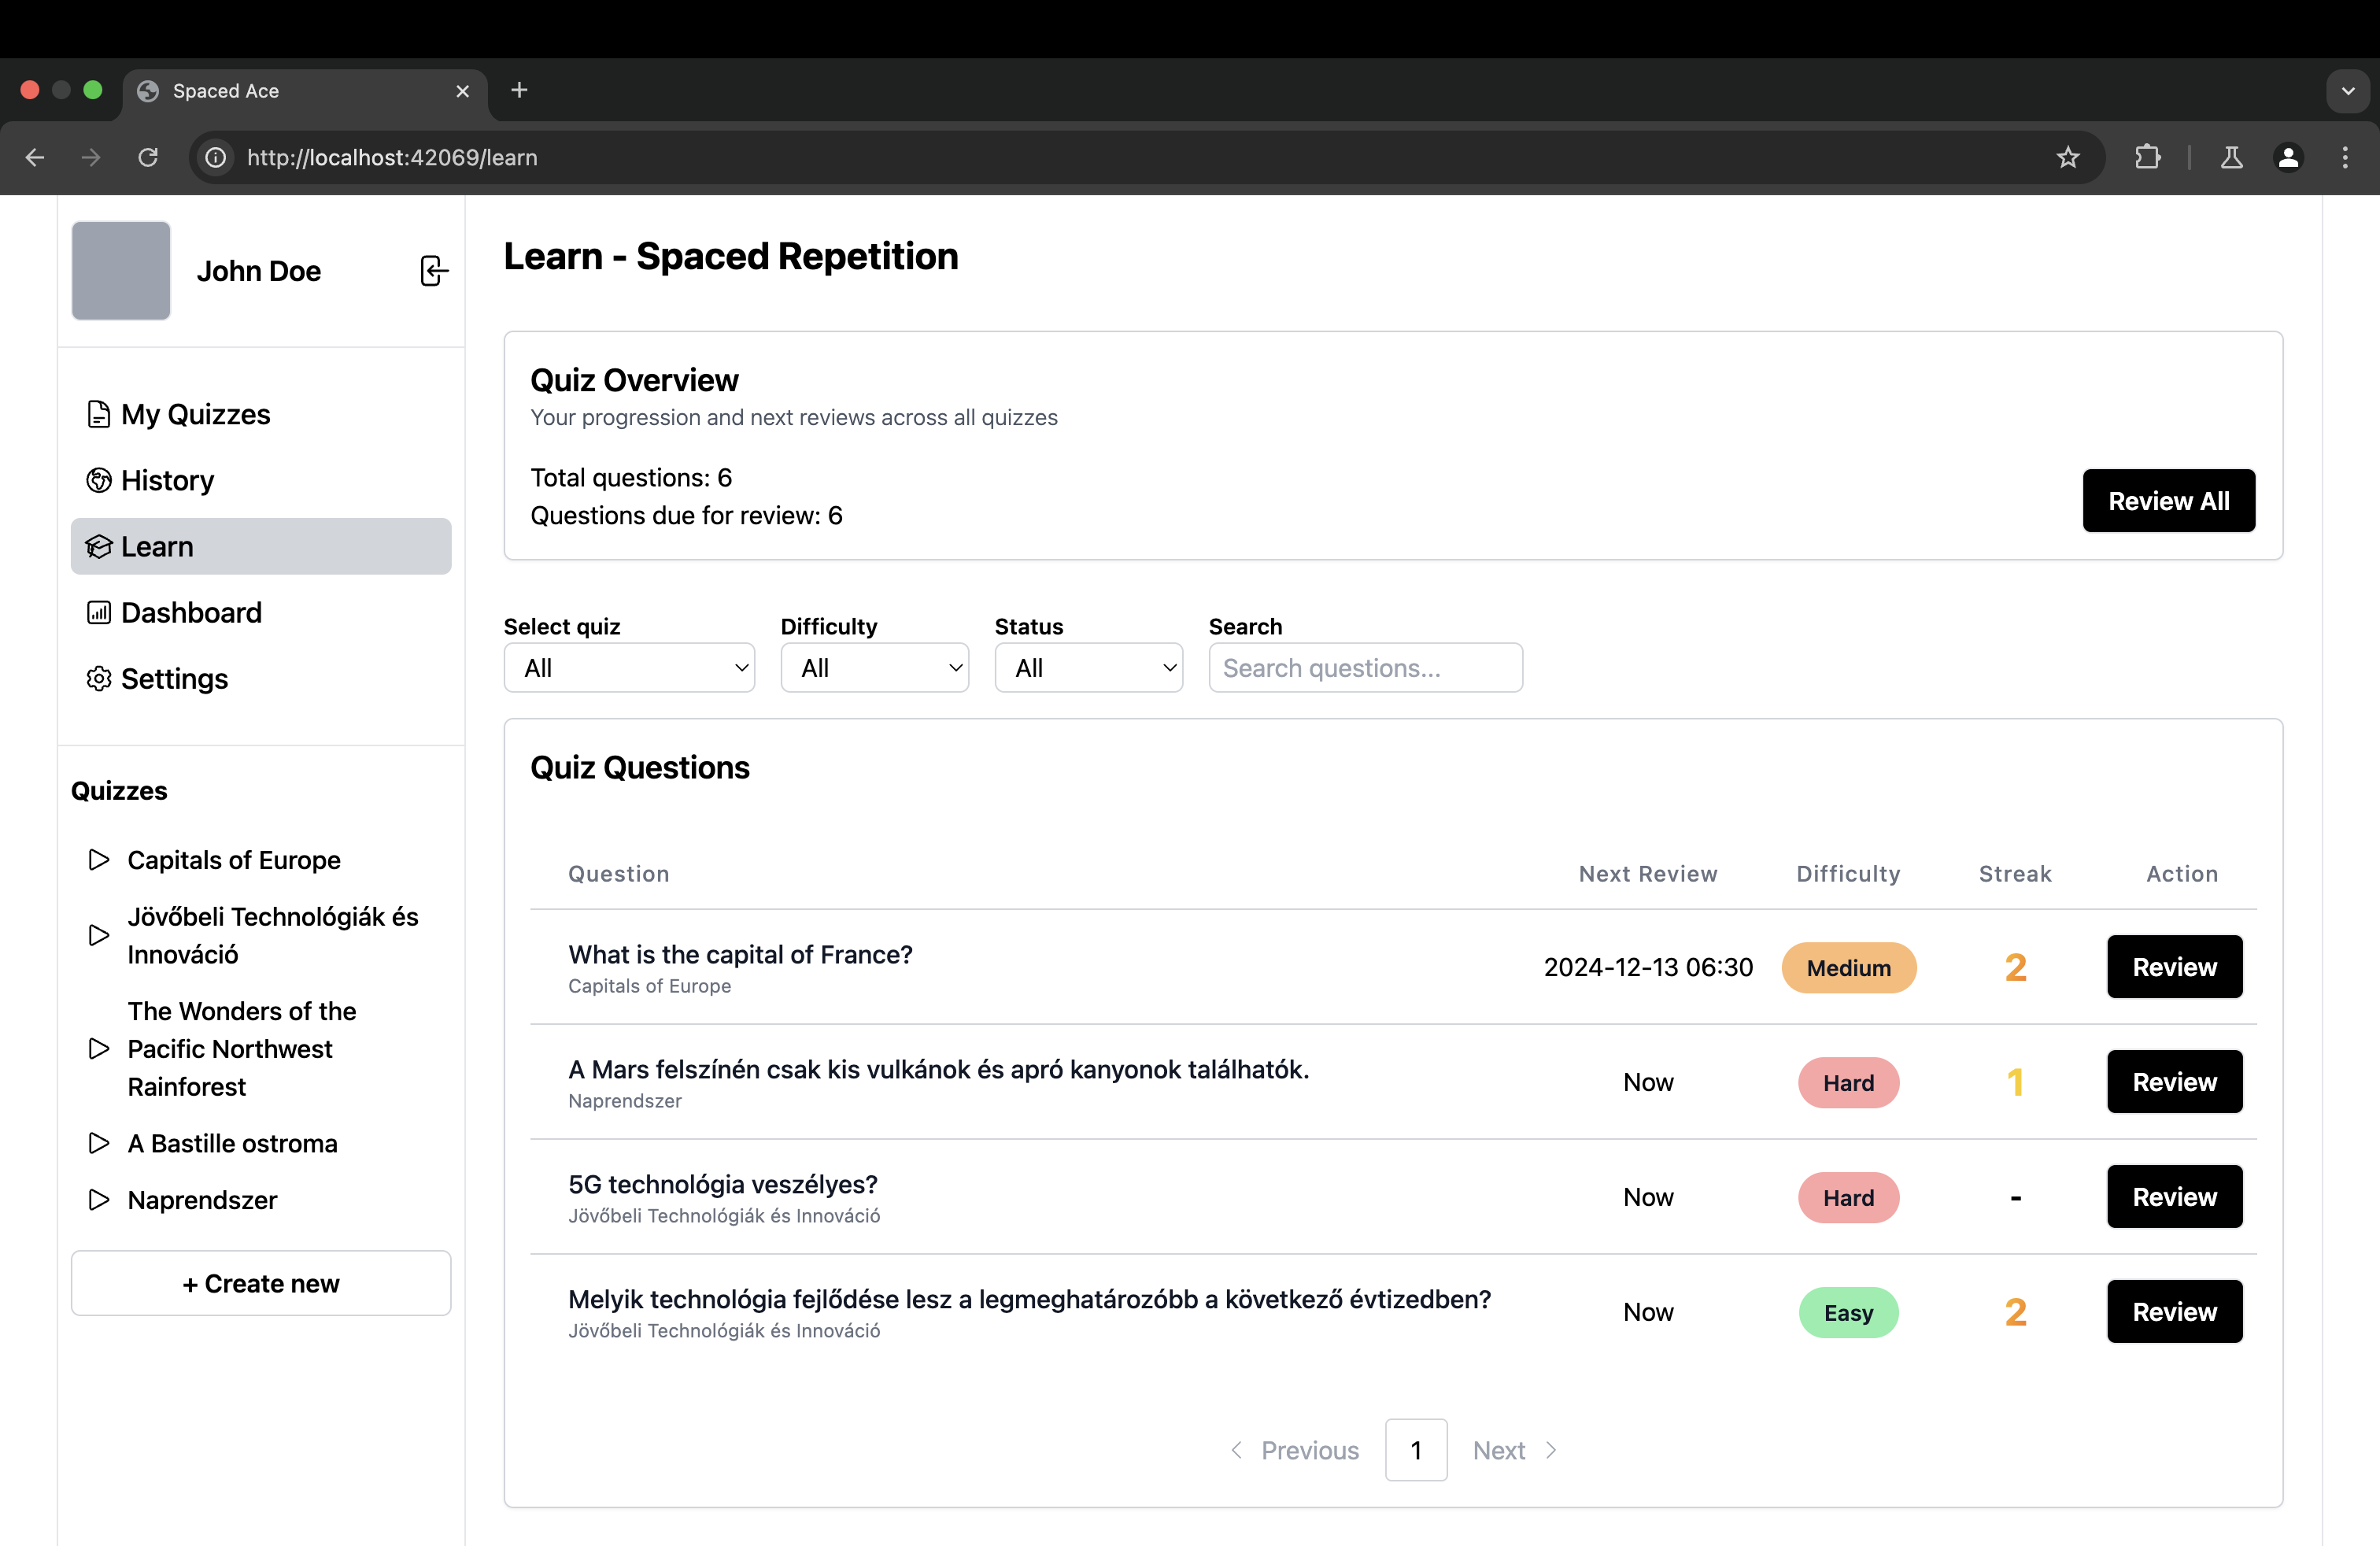
\includegraphics[width=0.9\textwidth, keepaspectratio]{figures/screenshot-learn-page.png}
	}
	\caption{Learn page}
	\label{fig:screenshot-learn-page}
\end{figure}

\subsection{Project structure}

The project follows a flat folder structure hierarchy inspired by \texttt{The Go Standard Project Layout}\footnote{https://github.com/golang-standards/project-layout}. Figure~\ref{fig:frontend-project-structure} shows this folder structure visually.

\begin{figure}[H]
    \centering
    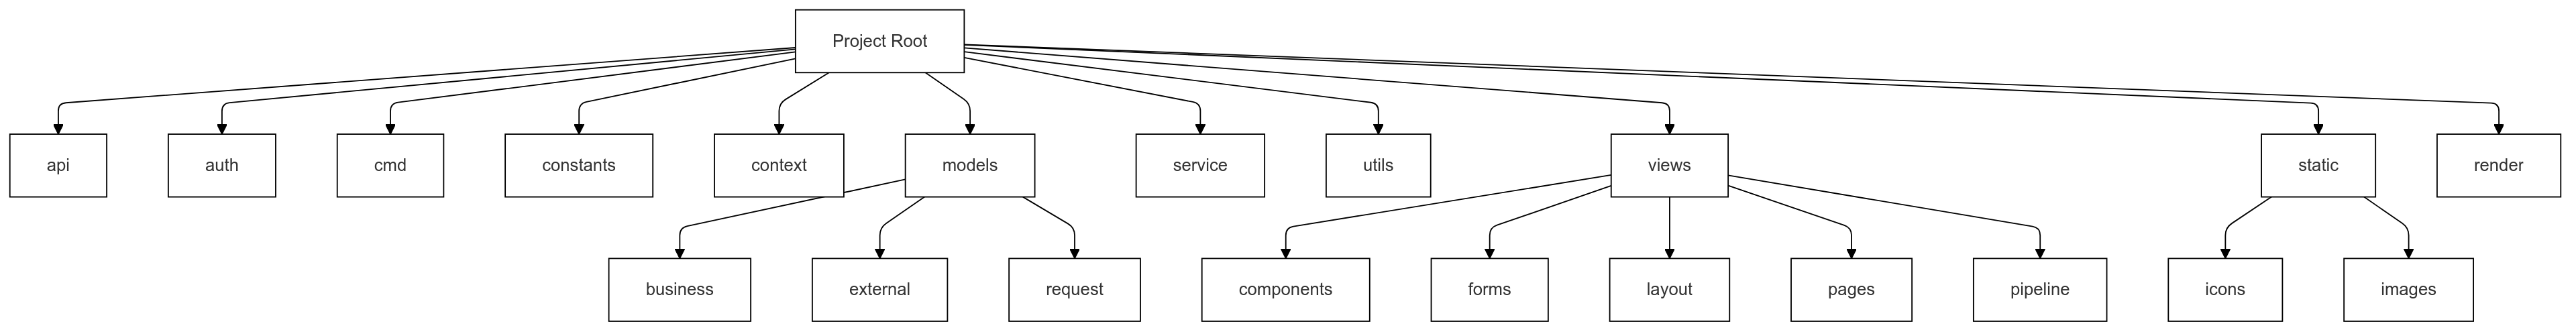
\includegraphics[width=0.9\textwidth, keepaspectratio]{figures/frontend-project-structure.png}
    \caption{Frontend project structure}
    \label{fig:frontend-project-structure}
\end{figure}

\textbf{api}: The \texttt{api} folder contains the endpoint handlers related to the pages and HTMX interactions.

\textbf{auth}: The \texttt{auth} folder contains the endpoint handlers related to the authentication function of the platform.

\textbf{cmd}: The folder \texttt{cmd} is a Go-specific folder containing the main functions. It is a common way to define the entry point of an application in \texttt{cmd/main.go}.

\textbf{constants}: The \texttt{constants} folder contains run-time constants; they wrap the provided environment variables and make them globally available for the application.

\textbf{context}: The \texttt{context} folder contains the custom context of the application. This context includes user information like a session ID and username.

\textbf{models}: The \texttt{models} folder contains Go representations of the data models in different layers and provides mappings between them. There are three layers of data: business, external, and request, which are separated into subfolders.

\textbf{service}: The \texttt{service} folder contains the ApiService, a proxy service providing access to the backend via function calls. This service is accessible through the custom context because the server calls usually require attaching the session ID to the request, and this service can do it automatically.

\textbf{utils}: The \texttt{utils} folder contains utils functions like generating gradient background from UUIDs and finding elements in lists.

\textbf{view}: The \texttt{view} folder contains the templ components and the generated Go code generated from them. They are also separated into subfolders based on their usage: \texttt{components}, \texttt{forms}, \texttt{layout}, \texttt{pages}, and \texttt{pipeline}.

\textbf{static}: The \texttt{static} folder is a regular webserver folder containing static resources for the application, such as scripts, images, and icons.

\textbf{render}: The \texttt{render} folder contains the configuration of the templ renderer and the render pipeline.

\subsection{Data models}

The application operates with three layers of data models. Each has a specific use case and can be mapped into other layer equivalents with mapping functions. These layers are the following: \texttt{business} used for doing the business logic, \texttt{external} used as Data Transfer Objects (DTO), and \texttt{request} used as communicating with the user. Listing~\ref{lst:mapping-example} shows an example for mapping a question object from \texttt{external} to \texttt{business} layer.

\begin{lstlisting}[caption=Mapping from external to business,label=lst:mapping-example]
func (a MultipleChoiceAnswer) MapToBusiness() (*business.MultipleChoiceAnswer, error) {
	return &business.MultipleChoiceAnswer{
		CommonAnswerData: business.CommonAnswerData{
			Id:         a.ID,
			SessionId:  a.SessionID,
			QuestionId: a.QuestionID,
			AnswerType: a.AnswerType,
		},
		Answers: strings.Split(a.Answers, ""),
	}, nil
}
\end{lstlisting}

The business layer objects are usually mappings from DTOs, with minor changes for effortless rendering. The DTOs are Go structs with \texttt{struct tags} used for parsing JSON objects. They are mostly the same as used on the backend. The request layer objects are similar to DTOs, but their \texttt{struct tags} help to map form data sent by the client instead of JSON sent by the server.

\subsection{Authentication}\label{subsec:frontend-authentication}

The authentication on the client side is an extension of the server-side version. The user sends the session cookie to the frontend, and the frontend server saves it in the execution context and uses it to fetch data from the backend. A custom context is created from the Echo context on each request by extending it with user-related information and instantiating an ApiService instance. The ApiService automatically attaches the session cookie to the requests before sending them to the backend. Listing~\ref{lst:session-middleware} shows the code of the custom session middleware.

\begin{lstlisting}[caption=Session middleware code,label=lst:session-middleware]
func SessionMiddleware(next echo.HandlerFunc) echo.HandlerFunc {
	return func(c echo.Context) error {
		cc := &AppContext{
			Context: c,
		}

		sessionCookie, err := c.Cookie("session")
		if err != nil {
			return next(cc)
		}

		cc.ApiService = service.NewApiService(sessionCookie)
		session, err := cc.ApiService.GetSession()
		if err != nil {
			return next(cc)
		}

		cc.Session = session
		cc.Set("cc", cc)
		return next(cc)
	}
}
\end{lstlisting}

The custom context creation and session checking are built on the Echo framework middleware feature. I defined a middleware that extends the Echo context and another that checks the extended context to contain the session information. The session creator middleware is placed before every request because it only tries extending the context, but the other one is placed before the execution of the authentication-required endpoint to ensure the user is authenticated. It works like the Angular web framework's Auth guard \footnote{https://angular.dev/api/router/CanActivate} feature. Listing \ref{lst:session-require-middleware} shows the middleware code that ensures the authentication.

\begin{lstlisting}[caption=Session checking middleware code,label=lst:session-require-middleware]
func RequireSessionMiddleware(next echo.HandlerFunc) echo.HandlerFunc {
	return func(c echo.Context) error {
		cc, ok := c.(*AppContext)
		if !ok || cc.Session == nil {
			return c.Redirect(http.StatusFound, "/login")
		}
		return next(c)
	}
}
\end{lstlisting}

\subsection{Rendering pipeline}

I designed a pipeline-like structure for rendering the components to make them easier to manage and use. The pipeline has three stages: two primary and one optional. These stages have different responsibilities and use cases, but they were a good addition to creating a well-organized render structure. The first stage determines the request type, the second renders the desired component(s), and the final extends the rendered component when necessary. The following figure~\ref{fig:rendering-pipeline} shows the whole rendering process.

\begin{figure}[H]
    \centering
    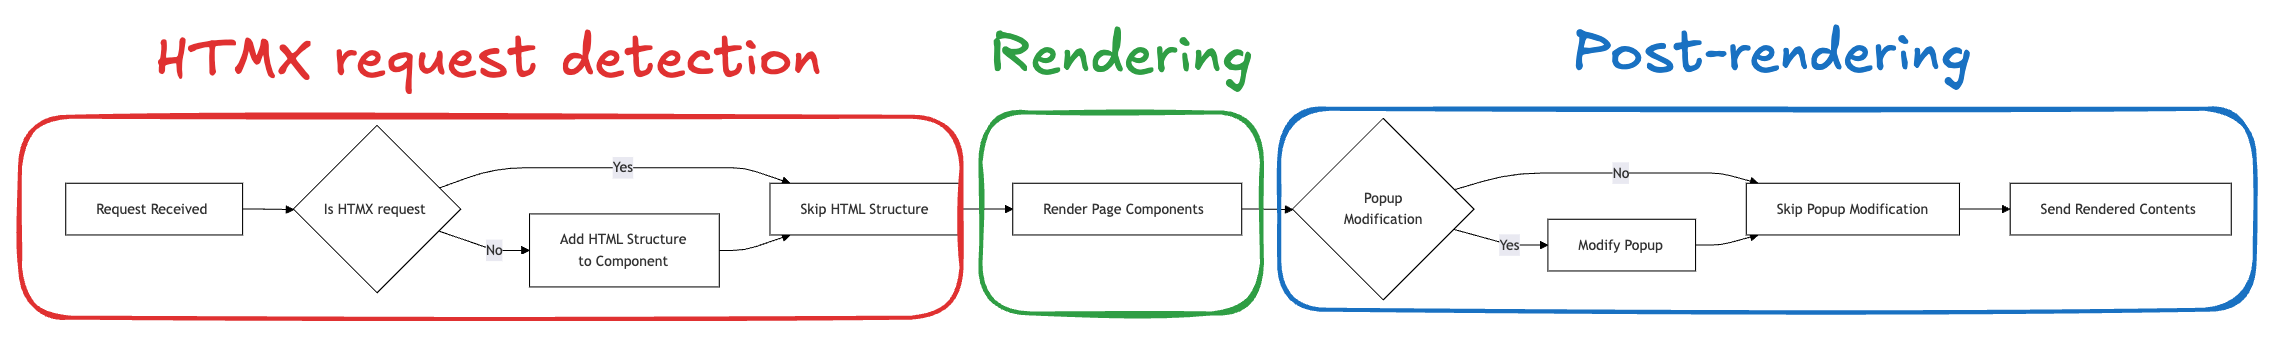
\includegraphics[width=0.9\textwidth, keepaspectratio]{figures/rendering-pipeline.png}
    \caption{Rendering pipeline}
    \label{fig:rendering-pipeline}
\end{figure}

The main problem was rendering the pages in a unified way for different needs. When a user navigates between pages, the frontend server should only render the page and the modified sidebar and let HTMX insert them into the DOM tree. However, when a user accesses a page directly with the URL, the server has to render a base HTML layout containing the scripts and styles in addition to the page and the sidebar—the pipeline's first stage checks whether the incoming request is a standard AJAX or an HTMX-boosted one.

The central stage of the pipeline is responsible for rendering the pages and components. It doesn't have to know whether a rendered element works as it is or is placed into a structure. This stage also allows additional components to be added, but it has to be done manually based on the use case. A common use case is using the HTMX OOB requests to update different parts of an application.

The final stage is responsible for automatically making post-render modifications. Currently, the only use case for this feature in the application is closing popups on navigation. It is made to be extendable, such as keeping a popup open, and can be set, but it has yet to be used.

\subsection{Form handling}

The HTMX requests contain information in HTTP forms. I used an interesting technique \footnote{https://www.youtube.com/watch?v=bQirFmhS3iw} for rendering and validating these forms in the application. The main idea is adding two parameters to the form components; the first is Go struct representing the values filled by the user, and the second is storing error messages. When a user submits a form, the frontend parses the values into the struct and validates them. If any error occurs or a value is inappropriate, the frontend server attaches error messages with keys to the error map and renders the component using the values and the messages. The following listing~\ref{lst:form-handling} shows the login form component's code and how the values and the error messages are set.

\begin{lstlisting}[caption=Login form,label=lst:form-handling]
templ LoginForm(errors map[string]string) {
	<form
		hx-post="/login"
		hx-swap="outerHTML"
		class="flex flex-col gap-y-4 p-6 w-[500px]"
	>
		<span class="text-center text-3xl font-bold">Login</span>
		@components.EMailInput(components.EMailInputProps{
			Error: errors["email"],
		})
		@components.TextInput(components.TextInputProps{
			Name:        "password",
			Label:       "Password",
			Placeholder: "Password",
			Type:        "password",
			Error:       errors["password"],
		})
		@components.Button(components.ButtonProps{
			Text: "Submit",
			Type: "submit",
		})
		@components.LinkButton("Sign up", "/signup", components.ButtonColorWhite)
		if errors["other"] != "" {
			<span class="w-full py-4 text-red-500 text-nowrap">{ errors["other"] }</span>
		}
	</form>
}
\end{lstlisting}

\subsection{Backend integration}

The frontend server makes HTTP requests to the backend endpoints using the ApiService from the context. ApiService is a proxy class that abstracts HTTP requests into function calls. It offers a unified and automated way to communicate with the backend. The session middleware constantly creates one instance for the current context containing the session information. The service's responsibility is to attach the session cookie to each request, and it manages by offering a common request sending and parsing function. This function takes the URL, HTTP method name, request, and response objects as parameters, creates a request, attaches the session cookie to the HTTP header, and processes the request. Listing~\ref{lst:api-service} shows the code of this util function.

\begin{lstlisting}[caption=ApiService code,label=lst:api-service]
func (a *ApiService) getResponse(method, path string, requestBody any, responseBody interface{}) error {
	data, err := json.Marshal(requestBody)
	if err != nil {
		return err
	}

	req, err := http.NewRequest(method, constants.BACKEND_URL+path, bytes.NewBuffer(data))
	if err != nil {
		return err
	}

	if a.sessionCookie != nil {
		req.AddCookie(a.sessionCookie)
	}

	resp, err := a.client.Do(req)
	if err != nil {
		return err
	}
	defer resp.Body.Close()

	if resp.StatusCode >= 400 {
		bodyBytes, err := io.ReadAll(resp.Body)
		if err != nil {
			return err
		}

		var result map[string]string
		err = json.Unmarshal(bodyBytes, &result)
		if err != nil {
			return err
		}

		return errors.New("error message: " + result["message"])
	}

	err = json.NewDecoder(resp.Body).Decode(&responseBody)
	if err != nil {
		return err
	}

	return nil
}
\end{lstlisting}

\section{Backend implementation}

 This section details the backend project, how the data is used, and how the authentication, database communication, or the spaced repetition algorithm are implemented. It focuses on highlighting the exciting and unique details of the implementation.

\subsection{Project structure}

The backend follows a flat folder structure hierarchy similar to the frontend with backend-specific features. This structure is a bit chaotic now, mainly due to using different SQL libraries.Figure~\ref{fig:backend-project-structure} shows the structure visually. Some parts, for example, config files, are missing from the figure because they are placed into the root, but this figure is about the folders.

\begin{figure}[H]
	\centering
	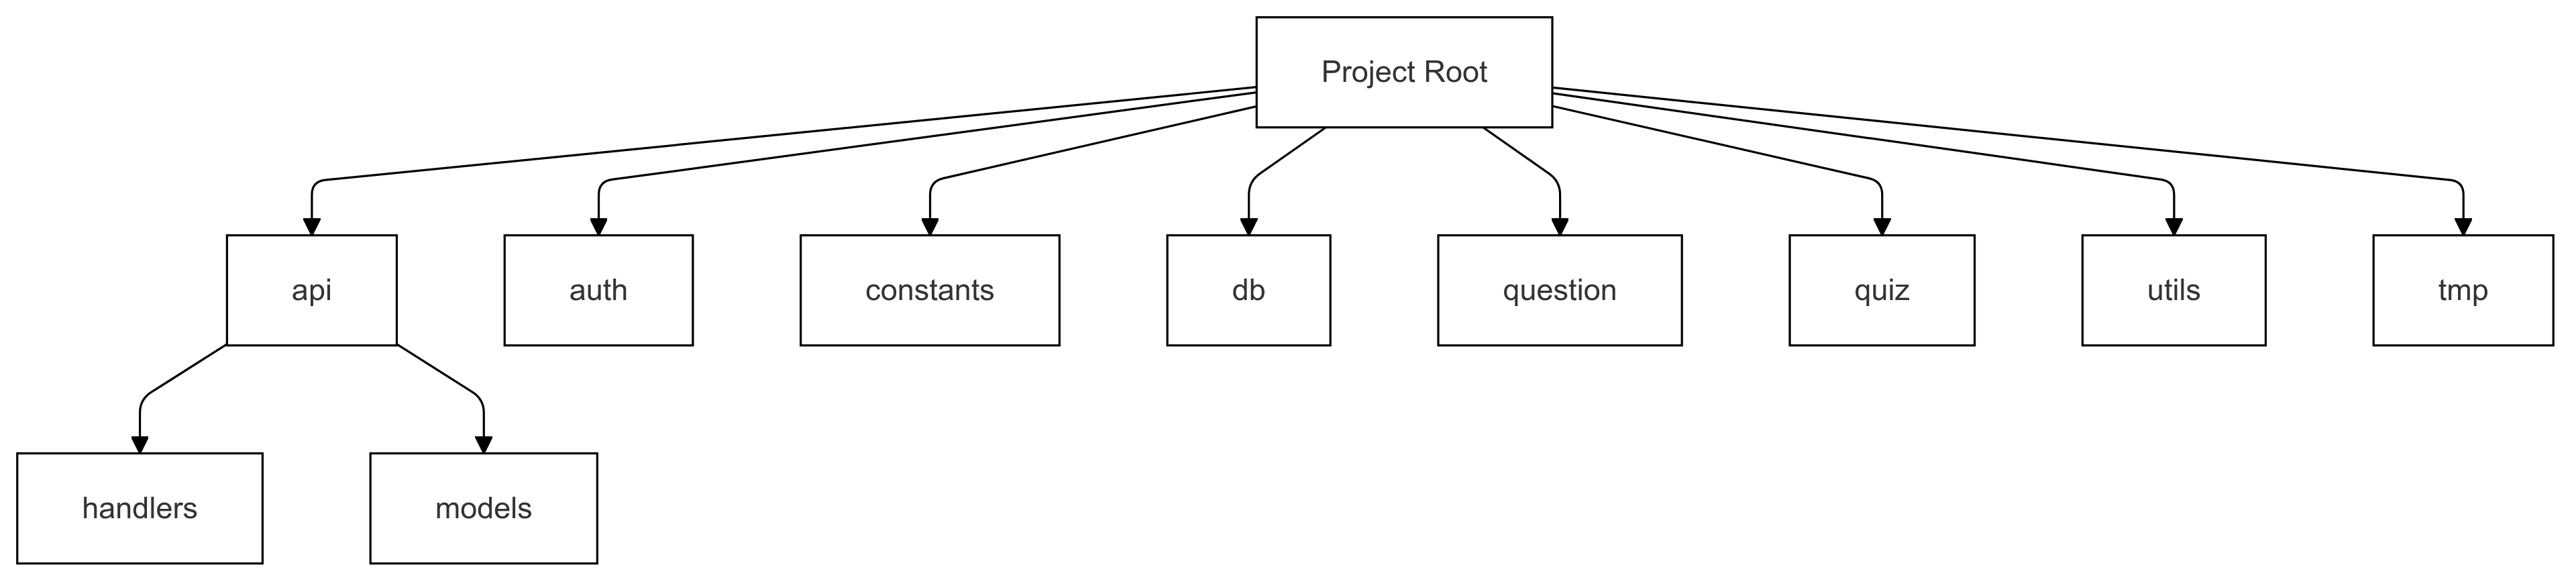
\includegraphics[width=0.8\textwidth, keepaspectratio]{figures/backend-project-structure.png}
	\caption{Backend project structure}
	\label{fig:backend-project-structure}
\end{figure}

\textbf{api}: The \texttt{api} folder contains the endpoint handlers and the DTO's. They are separated into two subfolders: \texttt{handlers} and \texttt{models}.

\textbf{auth}: The \texttt{auth} folder stores the authentication-related endpoint handlers, models, and database queries. These functions are placed here. They are implemented using the SQLx library.

\textbf{constants}: The \texttt{constants} folder is the same as in the fronted. It contains run-time constants and wraps environment variables into Go variables.

\textbf{db}: The \texttt{db} folder is a generated folder by SQLc, containing the SQL schemas, queries, and the glue code for accessing the database.

\textbf{question} and \textbf{quiz}: These two folders are for database codes and types used by the SQLx library, containing prepared statements and mapping types.

\textbf{utils}: The \texttt{utils} folder contains shared code for the application. Currently, they are database-related helper functions.

\textbf{tmp}: The \texttt{tmp} folder is a temporary folder containing the application's binary and related log files.

\subsection{Data models}

Unlike the frontend, backend data can be split into two layers: business and Data Access Object (DAO). In the case of the backend, the DTO and the business layer are merged. The business logic is performed on these objects containing the JSON parsing related \texttt{struct tags}. For now, it is sufficient, but I may need to separate them later.

The DAO layer contains the objects the database libraries use to map rows to the Go code. I do not apply them directly but map to their business layer equivalents to perform logic. There are two categories: the ones I wrote in Go for the SQLx library queries and the ones other SQL library generates. Listing~\ref{lst:sqlx-type} shows an example SQLx-compatible type struct declaration.

\begin{lstlisting}[caption=SQLx-compatible type struct declaration,label=lst:sqlx-type]
type DBSingleChoiceQuestion struct {
    UUID          string         `db:"uuid"`
    QuizID        string         `db:"quizid"`
    Question      string         `db:"question"`
    Answers       pq.StringArray `db:"answers"`
    CorrectAnswer string         `db:"correct_answer"`
}
\end{lstlisting}

\subsection{Authentication}

The platform uses session-based authentication with HTTP cookies. The frontend side of the implementation is discussed earlier in the frontend authentication subsection~\ref{subsec:frontend-authentication}. This subsection focuses on the backend side.

The implementation is straightforward; the service offers the endpoint \texttt{/authenticate-user}, where a user can submit the credentials, and the server creates a session. This session's ID is an HTTP cookie in the response and must be sent back by the client on every request. The session is currently stored in the database in the session table. It is automatically deleted after expiring due to the in-database chron job. Listing~\ref{lst:session-creation} shows the code for creating the session.

\begin{lstlisting}[caption=Session creation code,label=lst:session-creation]
func CreateSession(userId string) (string, error) {
	var id string
	err := utils.DB.Get(&id, "INSERT INTO sessions (id, user_id, valid_until) VALUES (gen_random_uuid(), $1, now() + interval '1 hour') RETURNING id", userId)
	if err != nil {
		return "", err
	}
	return id, nil
}
\end{lstlisting}

The server reads the session cookie and compares it to the value stored in the database to check the session. This check can be done automatically by a session-checking middleware or manually with Go code on the desired endpoints. When the user logs out, the server deletes its session from the database, preventing others from stealing it.

\subsection{SQLc implementation}

SQLc is the library for accessing the database with generated code from schemas and queries. The library generates the code from the given schema and query files using its configuration file. This file helps define the style of the generated code. Listing~\ref{lst:sqlc-config} shows the current config of the SQLc library.

\begin{lstlisting}[caption=SQLc configuration,label=lst:sqlc-config]
version: "2"
sql:
  - engine: "postgresql"
    queries: "query.sql"
    schema: "schema.sql"
    gen:
      go:
        package: "db"
        out: "db"
        sql_package: "pgx/v5"
        emit_result_struct_pointers: true
        emit_pointers_for_null_types: true
        overrides:
          - db_type: "uuid"
            nullable: false
            go_type:
              type: "string"
              pointer: false

          - db_type: "uuid"
            nullable: true
            go_type:
              type: "string"
              pointer: true

          - db_type: "pg_catalog.float8"
            nullable: false
            go_type: "float64"

          - db_type: "pg_catalog.float8"
            nullable: true
            go_type: "float64"

\end{lstlisting}

The library generates a \texttt{db.Quieries} object containing the generated function calling prepared statements. This object requires a database connection to work. I created a service called \texttt{SQLCQuerier} to link these to objects. This service is initiated in the main function before everything else and stored as a global object. This object is called everywhere in the application to perform database queries. Every query function requires a go context and query-related parameter struct for the inner prepared statement. The context is used to limit the lifetime of the query execution. It helps prevent infinity loads and memory leaks. The following listing~\ref{lst:sqlc-querier} shows an example of retrieving the SQLCQuerier object and performing a request using it.

\begin{lstlisting}[caption=Using the SQLCQuerier,label=lst:sqlc-querier]
	// Get the querier and create a Go context with lifetime of 5s
	sqlcQuerier := utils.GetQuerier()
	ctx, cancel := context.WithTimeout(context.Background(), 5*time.Second)
	defer cancel()

	// Get sessions from the database using the querier
	quizSessions, err := sqlcQuerier.GetQuizSessionsByUserId(ctx, userID)
	if err != nil {
		return echo.NewHTTPError(http.StatusInternalServerError, fmt.Errorf("error getting quiz sessions for user: %w", err))
	}
\end{lstlisting}

\subsection{Spaced repetition algorithm}\label{subsec:spaced-repetition-algorithm}

The spaced repetition learning algorithm schedules the user's learning materials. It uses historical data gathered and stored in question-answering. When a user adds a quiz to its learning list, the platform finds the questions from the quiz and creates an immediate schedule with default values. It makes available the platform to check the user's answers and reschedule the questions based on the concrete answers.

The algorithm's implementation is straightforward; it consists of one function and a few lines of code. The functions take a review item and a score percentage as parameters and return the review item with the scheduled values. The review item represents a card used in the spaced repetition, and the score percentage is the score they got for the given question. The algorithm scales up the score between 1 and 5 for later calculations. Then, the score is higher than 3, meaning the user answered correctly with difficulties, or below it, meaning the answer needs to be corrected. Then, the algorithm calculates the difficulty, the ease factor, and the new schedule for the question. Finally, it stores the modified item and shows it to the user. Listing~\ref{lst:spaced-repetition} shows the concrete implementation of the algorithm written in Go.

\begin{lstlisting}[caption=Spaced repetition algorithm written in Go,label=lst:spaced-repetition]
func applySpacedRepetitionAndStore(ctx context.Context, reviewItem *models.ReviewItem, percentage float64) (*models.ReviewItem, error) {
	// score is the user's performance rating, where:
	// 5 = perfect recall, 4 = correct with minor hesitation, 3 = correct but difficult,
	// 2 = incorrect, but partially remembered, 1 = completely incorrect
	score := 5 * percentage

	if score >= 3 {
		reviewItem.Difficulty = math.Max(1, reviewItem.Difficulty-1)

		if reviewItem.Streak == 0 {
			reviewItem.IntervalInMinutes = 60
		} else if reviewItem.Streak == 1 {
			reviewItem.IntervalInMinutes = 3 * 60
		} else {
			reviewItem.IntervalInMinutes = int32(float64(reviewItem.IntervalInMinutes) * reviewItem.EaseFactor * (1 / reviewItem.Difficulty))
		}

		reviewItem.EaseFactor = reviewItem.EaseFactor + (0.1 - (5-score)*0.08)
		reviewItem.Streak = reviewItem.Streak + 1
	} else {
		reviewItem.Difficulty = math.Min(5, reviewItem.Difficulty+1.5)

		reviewItem.IntervalInMinutes = 60

		reviewItem.EaseFactor = math.Max(1.3, reviewItem.EaseFactor-0.2)
		reviewItem.Streak = 0
	}

	reviewItem.NextReviewDate = models.NullableTime{
		Time: reviewItem.NextReviewDate.Time.Add(time.Duration(reviewItem.IntervalInMinutes) * time.Minute),
	}

	// store the data ...

	return reviewItem, nil
}
\end{lstlisting}

\subsection{AI integration}

The AI features are found in different services but are available from the backend. They generate questions of a given type from the user-provided context. This context is usually several paragraphs long, so the server needs to split it into smaller parts. It not only speeds up the generation but also makes it more controllable. Máté made a simple algorithm for splitting up the context and iterating between the parts with a round-robin algorithm.

When a user submits long text as a question context, the server calculates a hash for later identification and splits it recursively into 2-3 paragraph chunks. For the first time, the first chunk and the question type are sent to the LLM API, which takes care of the generation. Next time, the server will check the hash and find the next chunk for the generation. These chunks are stored in the database and cached in memory to optimize retrieval speed.

The questions return from the LLM API as JSON objects in HTTP responses. The generation usually takes several seconds to finish; until then, the server and client have to wait. As I wrote this thesis, Máté and I started considering implementing HTTP streams besides the current method, allowing the client to show partially generated questions. This concept is more complicated than the implemented one and would need changes in every layer. This idea could be excellent for improving the overall user experience.